\documentclass[../Head/Main.tex]{subfiles}
\begin{document}
\section{Segmentation of Images}
The code described in this section is found in the file .\\
Four methods of segmentation are considered for distinguishing the orange pumpkins from the green background:
\begin{itemize}
\item Segmentation based on a range of RGB values
\item Segmentation based on a range of CieLAB values
\item Segmentation by histogram backprojection
\item Segmentation by a maximum euclidean distance from the mean RGB value
\end{itemize}

\subsection{Segmentation by Range of RGB Color Values}
The simplest method for segmentation to be applied is by only including pixels that are within some predefined color range. The range must be defined so as to include as much as possible of the pumpkin color range and exclude as much as possible of the color range in the remainder of the image.\\
Defining the allowed range for the different color channels was approached by examining the results of the color analysis described in section \ref{sec:colorAnalysis}. By looking at the histograms figure \ref{fig:histRgb} a proper lower boundary for all three RGB color channels would be the mean value minus one standard deviation and the upper boundary could be set to the mean value plus two standard deviations. In this way, the colors of the pumpkins would be approximately seperated from the remaining colors without too much overlap. Part of the segmented image drawed back on the original image can be seen in figure \ref{fig:bgrSeg}.

\begin{figure}[H]
\centering
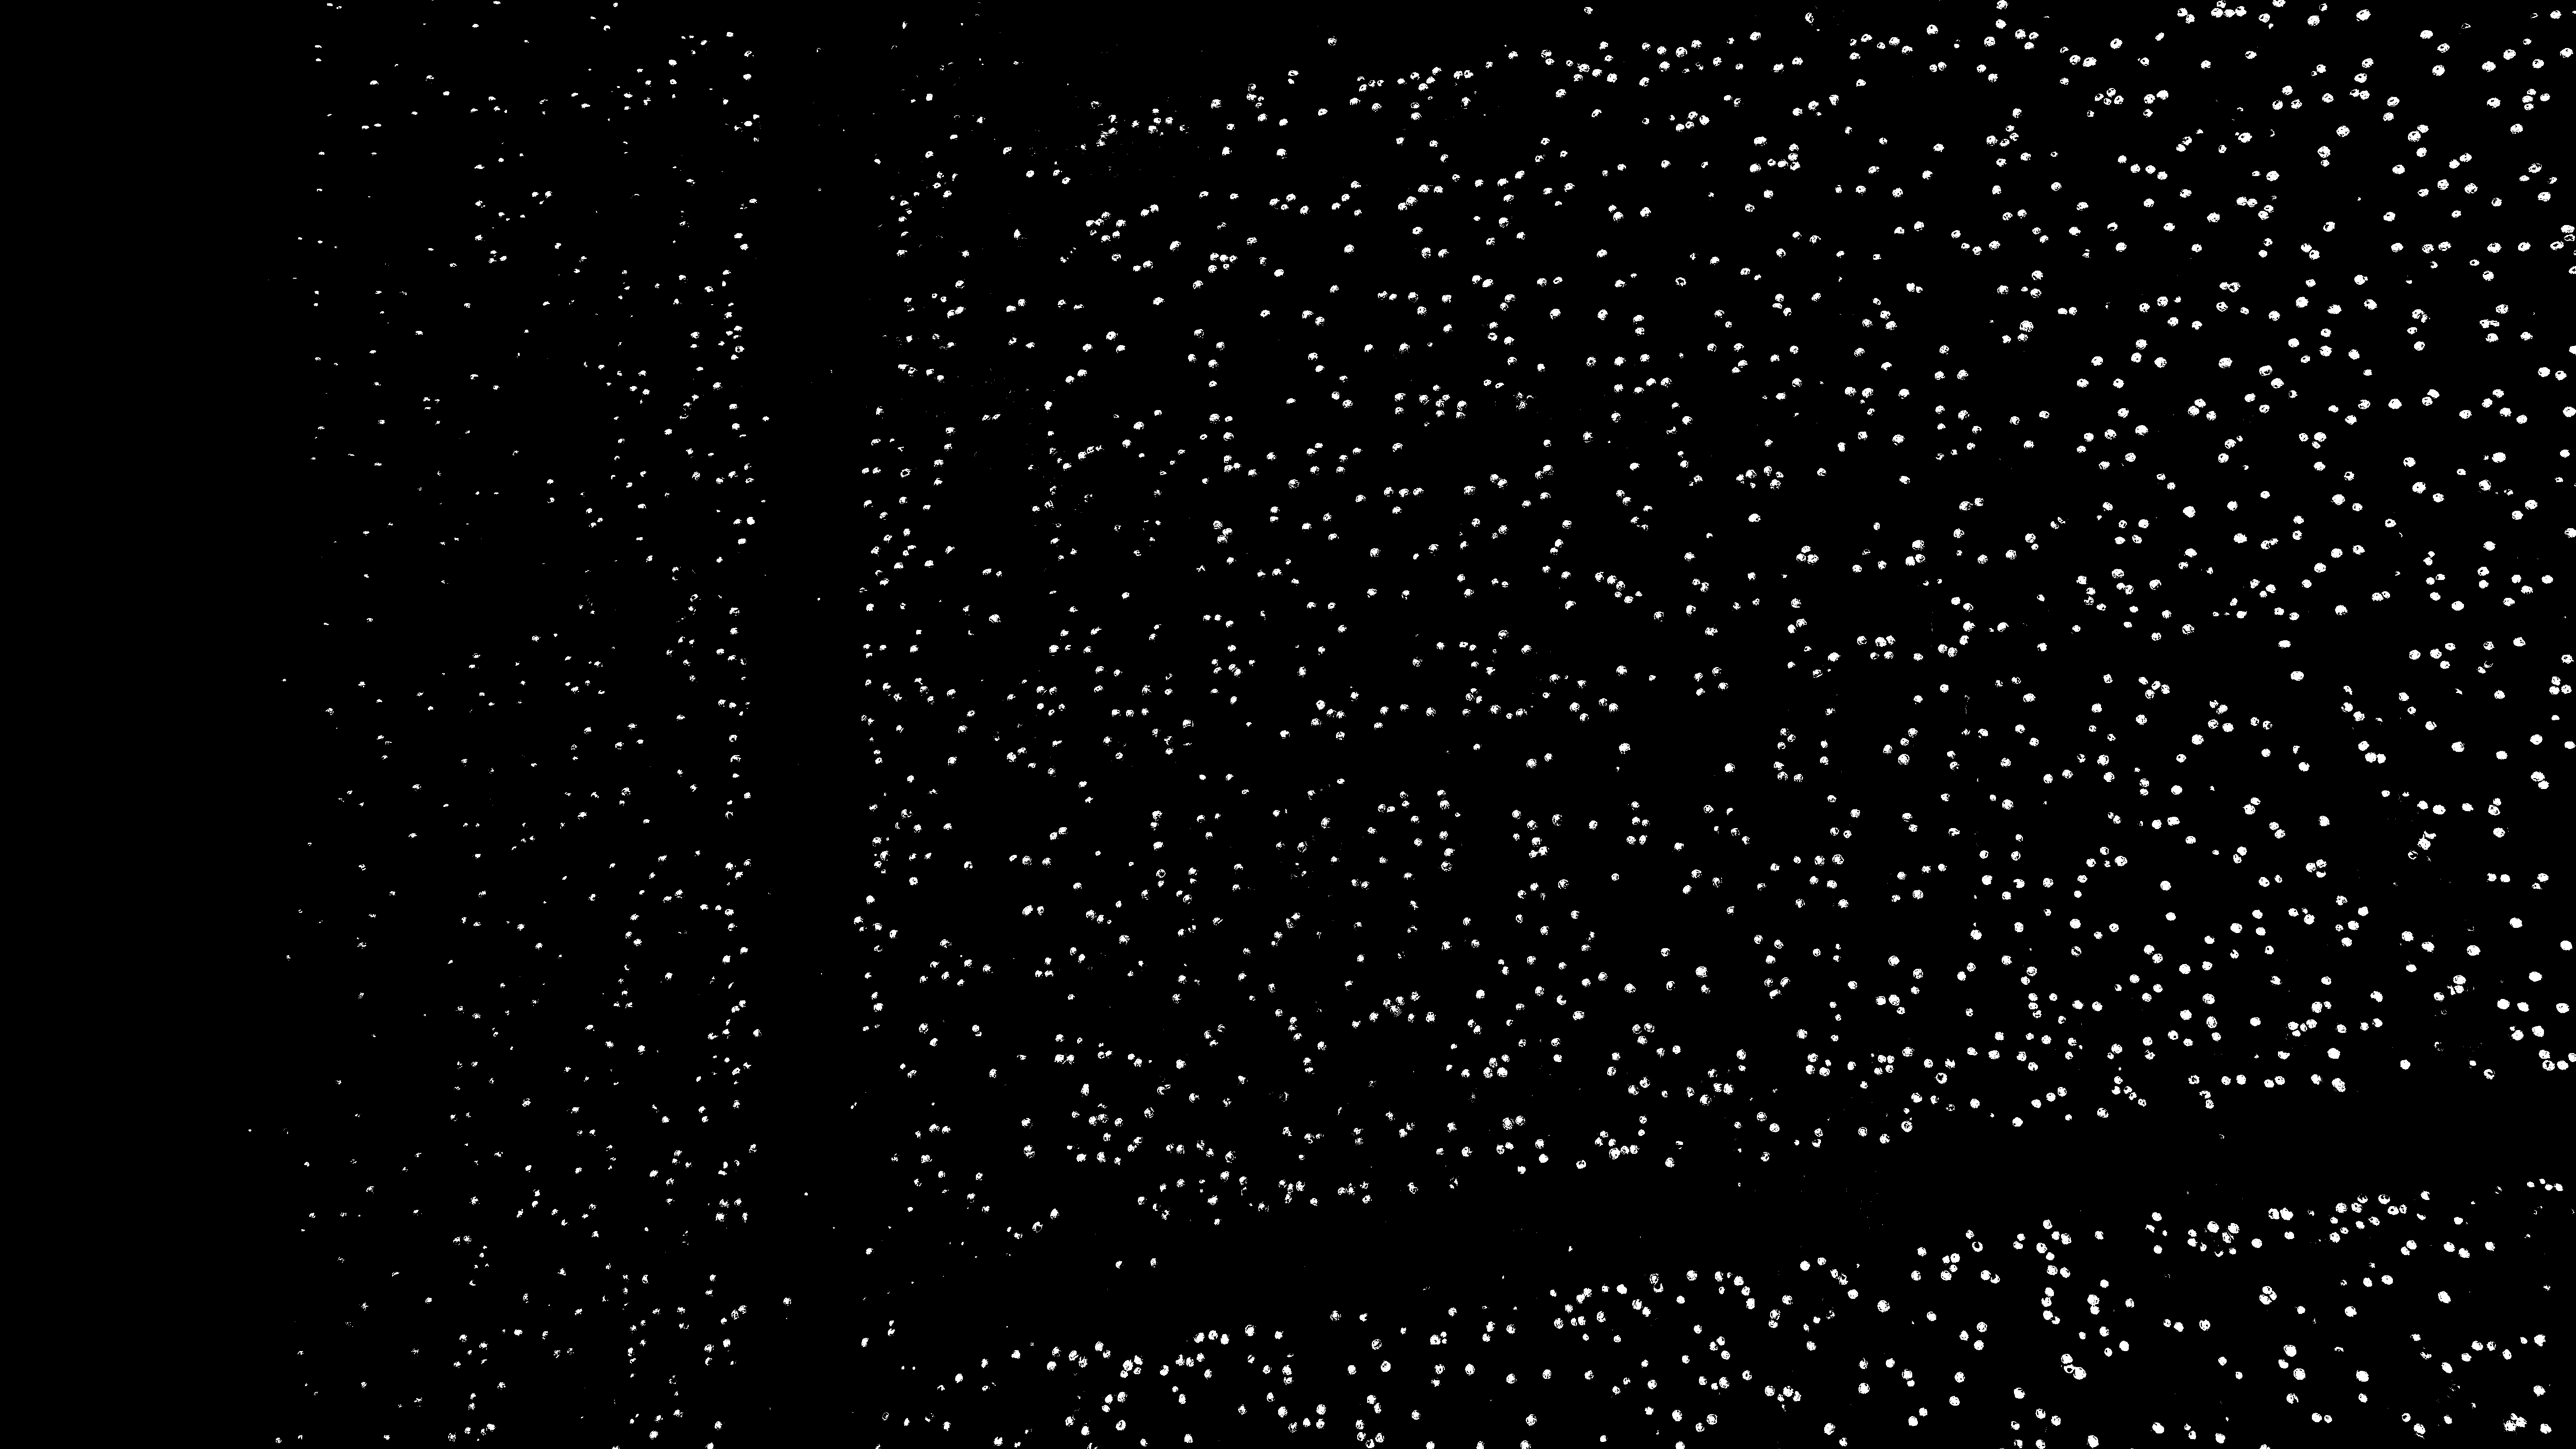
\includegraphics[width=0.8\textwidth]{../Figures/ex2_bgr_inrange.png}
\caption{Segmentation by range of BGR values}
\label{fig:bgrSeg}
\end{figure}

From visual inspection it can be seen that the RGB range segmentation segments the image quite well. 

\subsection{Segmentation by Range of CieLAB Color Values}
The same approach as segmentation by RGB color ranges is applied for the image converted to the CieLAB color space. By inspection of \ref{fig:histLab}, appropriate lower and upper boundaries of the color ranges are the mean value minus one standard deviation and the mean value plus two standard deviations. This will once again seperate the colors of the pumpkins from the color characteristics of the entire image. Part of the segmented image drawed back on the original image is seen in figure \ref{fig:labSeg}.

\begin{figure}[H]
\centering
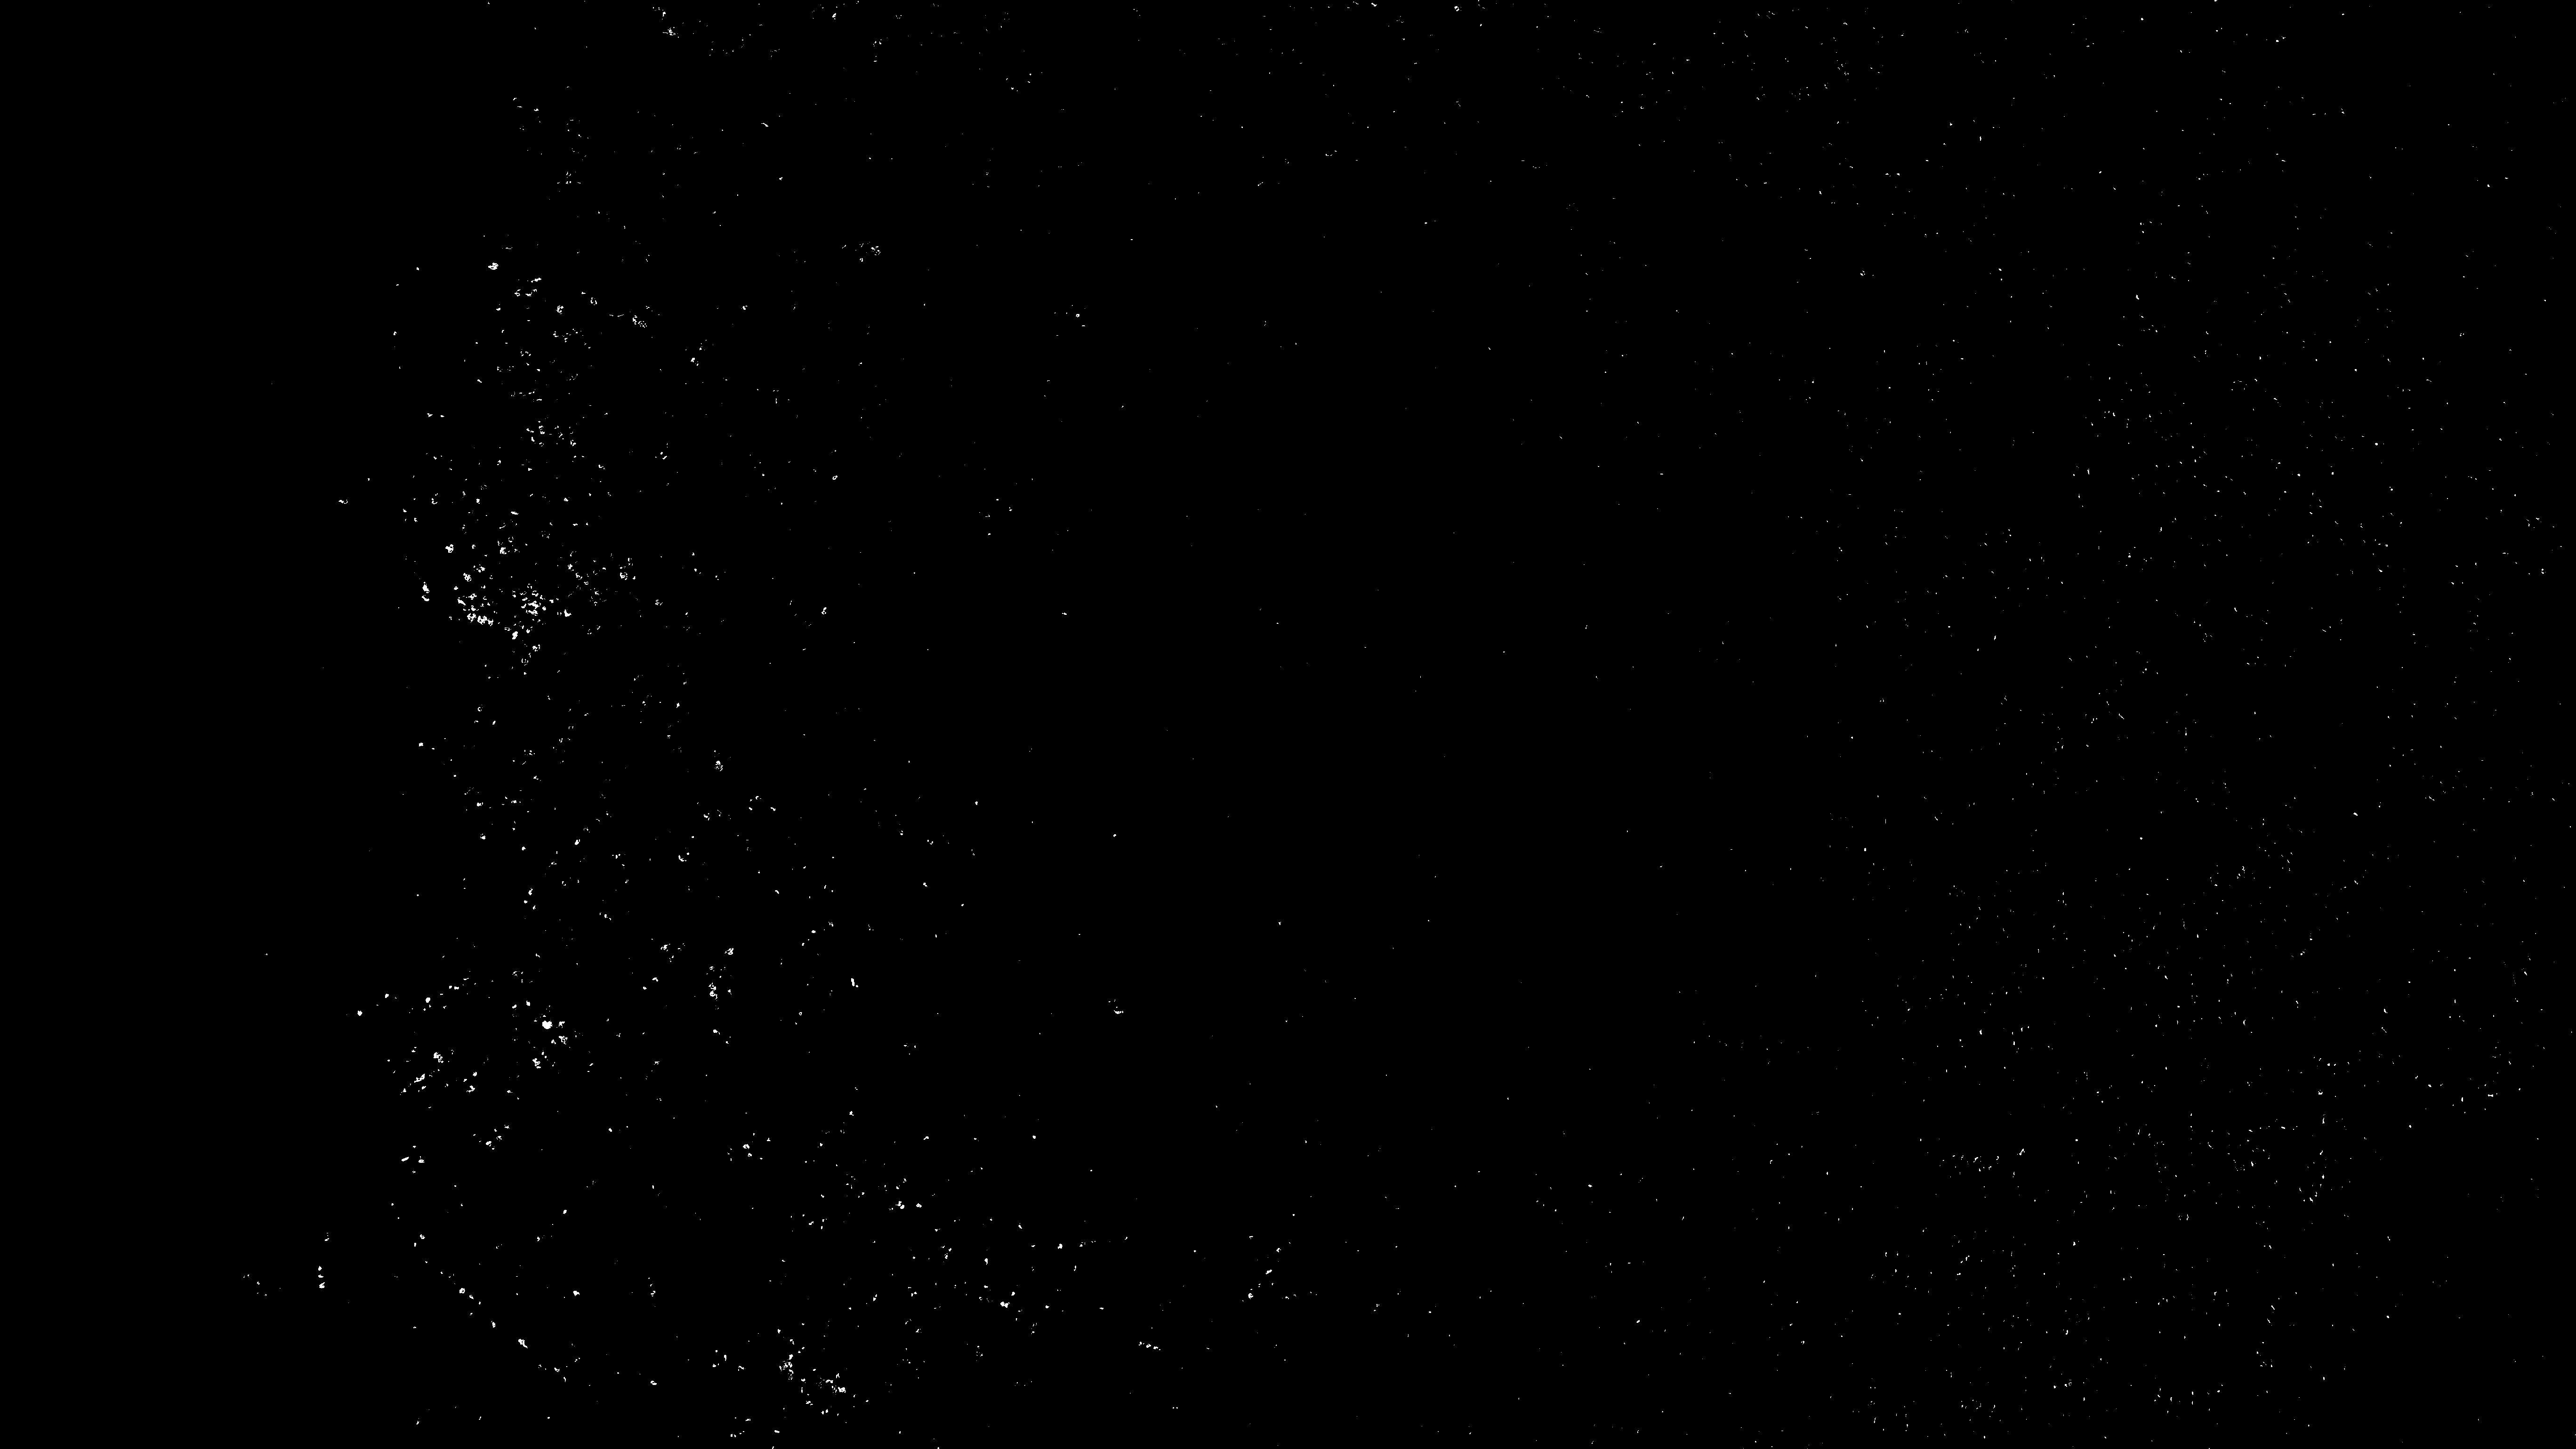
\includegraphics[width=0.8\textwidth]{../Figures/ex2_lab_inrange.png}
\caption{Segmentation by range of CieLAB values}
\label{fig:labSeg}
\end{figure}

Using the color information of the pixels, we can estimate if they are pumpkin or not.
The simplest way to do that is to check if the color values fall inside a predetermined range.

To get usable results, we need to choose the limits wisely.
We did that by looking at the histograms of the color channels in the original image.
In the ranges we used the mean +- one standard deviation.

Slight natural variations in color can cause big differences in the performance of our detection.
In order to get a more consistent look on the pumpkins we used a blurring algorithm.
Our choice of algorithm is median blur. It performs nicely in terms of smoothing while also keeping hard contours.

Here is a showcase of the filter in action. Original (left) and filtered (right). The filter kernel size is set to 9 pixels.

.. image:: images/ori_smol.jpg
    :width: 49 %
.. image:: images/blurred_smol.jpg
    :width: 49 %


\end{document}